\section*{Data Overview}
The primary data for this study is sourced from the comprehensive battery cycling datasets hosted on data.matr.io. The consolidated dataset consists of 169 Lithium-ion phosphate (LFP) cells cycled under varying fast-charging conditions. These cells represent 61 distinct average charging C-rates, providing various degradation profiles and cycle lifetimes.

\subsection*{Data Structure and Extraction}
The raw data, originally stored in MATLAB format, was ingested into a Python-based workflow for analysis. This process followed (authors and citation)'s process outlined in their GitHub. 
\begin{description}
    \item[Cell Level:] Each battery is indexed by a unique key. The keys map to a dictionary containing the \texttt{cycle\_life}, \texttt{charge\_policy}, \texttt{summary}, and \texttt{cycles}.
    \item[Summary Level:] High-level features are tracked each cycle, including Internal Resistance (IR), charge time, charge and discharge capacity ($Q_c$, $Q_d$), and temperature metrics ($T_{avg}$, $T_{min}$, $T_{max}$).
    \item[Cycle Level:] Time-series measurements within individual cycles provide charge and discharge capacity, linear interpolated discharge capacity, temperature, linear interpolated temperature, voltage, and derived vectors of discharge.
\end{description}

The \texttt{cycle\_life} indicates the number of cycles until end of life (EoL) is reached, while the \texttt{charge\_policy} indicates the specific charging protocol used for that cell.

\subsection*{Data Dictionary}

% Table 1: Cell Level
\begin{table}[h]
\centering
\caption{Cell Level Variables}
\label{tab:cell_level}
\begin{tabular}{lll}
\toprule
Variable & Description & Type \\
\midrule
\texttt{cycle\_life} & Number of cycles until EoL & Float \\
\texttt{charge\_policy} & Charging protocol & String \\
\texttt{summary} & Metadata for each cycle & Dictionary \\
\texttt{cycles} & Time series of measurements & Dictionary \\
\bottomrule
\end{tabular}
\end{table}

% Table 2: Summary Level
\begin{table}[h]
\centering
\caption{Summary Level (Cycle-by-Cycle Metadata)}
\label{tab:summary_level}
\begin{tabular}{lll}
\toprule
Variable & Description & Type \\
\midrule
\texttt{IR} & Internal resistance & Numeric array \\
\texttt{QC} & Charge capacity & Numeric array \\
\texttt{QD} & Discharge capacity & Numeric array \\
\texttt{Tavg} & Average temperature & Numeric array \\
\texttt{Tmin} & Minimum temperature & Numeric array \\
\texttt{Tmax} & Maximum temperature & Numeric array \\
\texttt{chargetime} & Charge time & Numeric array \\
\texttt{cycle} & Cycle number & Numeric array \\
\bottomrule
\end{tabular}
\end{table}

% Table 3: Cycle Level
\begin{table}[h!]
\centering
\caption{Cycle Level (Intra-cycle Time Series)}
\label{tab:cycle_level}
\begin{tabular}{lll}
\toprule
Variable & Description & Type \\
\midrule
\texttt{I} & Current & Numeric array \\
\texttt{Qc} & Charge capacity & Numeric array \\
\texttt{Qd} & Discharge capacity & Numeric array \\
\texttt{Qdlin} & Linear interpolated discharge capacity & Numeric array \\
\texttt{T} & Temperature & Numeric array \\
\texttt{Tdlin} & Linear interpolated temperature & Numeric array \\
\texttt{V} & Voltage & Numeric array \\
\texttt{dQdV} & Derived vectors of discharge & Numeric array \\
\texttt{t} & Time & Numeric array \\
\bottomrule
\end{tabular}
\end{table}

\subsection*{Data Partitioning and Grouping Logic}
Zhou and Howey (2023) partitioned the data into eight groups based on their cycling conditions and calculated the variance partition coefficient (VPC). Specifically, they calculated:

\begin{align*}
\text{VPC} &= \frac{\sigma^2_{\text{group}}}{\sigma^2_{\text{individual}} + \sigma^2_{\text{group}}} \\
\sigma^2_{\text{group}} &= \text{var}\left(\bar{u}_j - \bar{u}\right), \quad \bar{u} = \frac{1}{N} \sum_{j=1}^{k} \sum_{i=1}^{n_j} y_{ji} \\
\sigma^2_{\text{individual}} &= \text{var}\left(y_{ji} - \bar{u}_j\right), \quad \bar{u}_j = \frac{1}{n_j} \sum_{i=1}^{n_j} y_{ji}
\end{align*}

where $\sigma^2_{\text{group}}$ represents lifetime variance between groups and $\sigma^2_{\text{individual}}$ represents the total within-group lifetime variance. They obtained a VPC of 74.5\%, implying that between-group variance accounts for the majority of total lifetime variance. 

\subsection*{Grouping Results}
Following Zhou and Howey (2023), we first applied constrained K-means clustering on average charging C-rate. While this produced groups with low within-group C-rate variance (see Figure 1), the resulting VPC was only 38.973\%. We subsequently grouped cells by their unique charging policy string and optimized via a hill-climbing algorithm to achieve a VPC of 74.406\%. The hill-climb grouping exhibits higher within-group C-rate variance but lower within-group EoL variance (see Figure 2).

\begin{figure}[H]
    \centering
    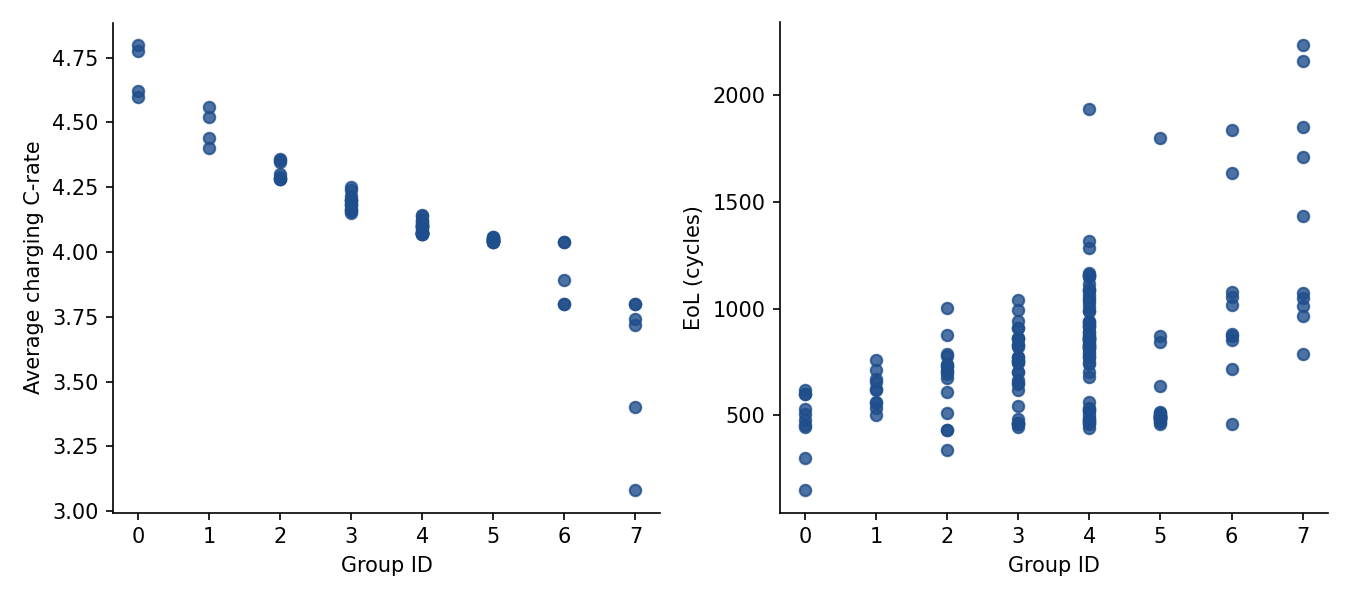
\includegraphics[width=0.8\textwidth]{fig4_km_group_crate_eol} 
    \caption{Distribution of average charging C-rate and EoL for each group obtained from constrained K-means.}
    \label{fig:battery_data}
\end{figure}
\begin{figure}[H]
    \centering
    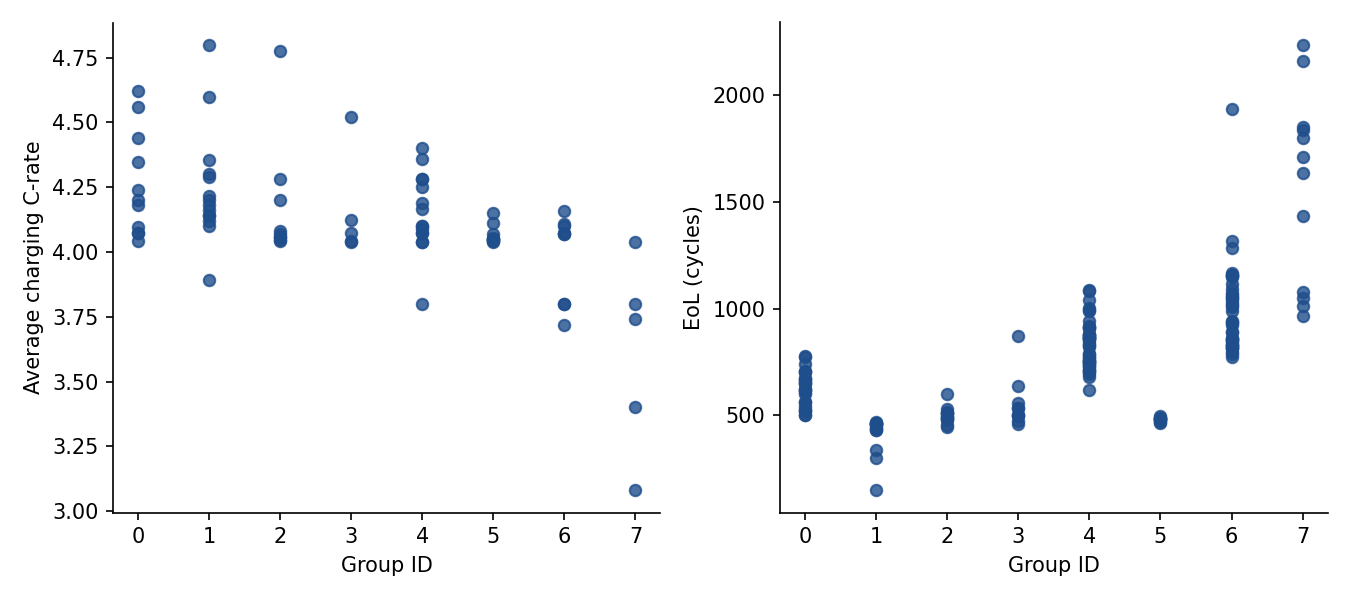
\includegraphics[width=0.8\textwidth]{fig4_group_crate_eol} 
    \caption{Distribution of average charging C-rate and EoL for each group obtained from hill-climb optimization.}
    \label{fig:battery_data}
\end{figure}